% Created 2020-06-22 lun. 13:27
% Intended LaTeX compiler: pdflatex
\documentclass{ISMA_USD2020}
\usepackage[utf8]{inputenc}
\usepackage[T1]{fontenc}
\usepackage{graphicx}
\usepackage{grffile}
\usepackage{longtable}
\usepackage{wrapfig}
\usepackage{rotating}
\usepackage[normalem]{ulem}
\usepackage{amsmath}
\usepackage{textcomp}
\usepackage{amssymb}
\usepackage{capt-of}
\usepackage{hyperref}
\usepackage[most]{tcolorbox}
\usepackage{bm}
\usepackage{booktabs}
\usepackage{tabularx}
\usepackage{array}
\usepackage{siunitx}
\usepackage{amsmath,amssymb,amsfonts, cases}
\usepackage{algorithmic, graphicx, textcomp}
\usepackage{xcolor, import, hyperref}
\usepackage[USenglish, english]{babel}
\setcounter{footnote}{1}
\input{config.tex}
\author[1,3] {T. Dehaeze}
\author[1,2] {C. Collette}
\affil[1] {Precision Mechatronics Laboratory\NewLineAffil University of Liege, Belgium \NewAffil}
\affil[2] {BEAMS Department\NewLineAffil Free University of Brussels, Belgium \NewAffil}
\affil[3] {European Synchrotron Radiation Facility \NewLineAffil Grenoble, France e-mail: \textbf{thomas.dehaeze@esrf.fr}}
\bibliographystyle{IEEEtran}
\date{}
\title{Active Damping of Rotating Positioning Platforms}
\begin{document}

\maketitle

\abstract{
    Abstract text to be done
}

\section{Introduction}
\label{sec:orgd20252d}
\label{sec:introduction}
\cite{dehaeze18_sampl_stabil_for_tomog_exper}

\section{System Under Study}
\label{sec:orgacbe1ae}
\subsection{Rotating Positioning Platform}
\label{sec:org07e4fc8}
Consider the rotating X-Y stage of Figure \ref{fig:rotating_xy_platform}.

\begin{itemize}
\item \(k\): Actuator's Stiffness [N/m]
\item \(m\): Payload's mass [kg]
\item \(\Omega = \dot{\theta}\): rotation speed [rad/s]
\item \(F_u\), \(F_v\)
\item \(d_u\), \(d_v\)
\end{itemize}

\begin{figure}[htbp]
\centering
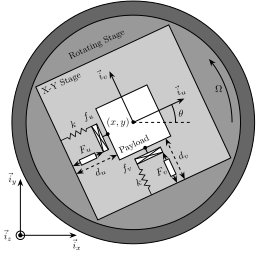
\includegraphics[scale=1]{figs/rotating_xy_platform.pdf}
\caption{\label{fig:rotating_xy_platform}Figure caption}
\end{figure}


\begin{figure}[htbp]
\centering
\includegraphics[width=0.5\linewidth]{figs/cedrat_xy25xs.jpg}
\caption{\label{fig:cedrat_xy25xs}Figure caption}
\end{figure}

\subsection{Equation of Motion}
\label{sec:orgac1a52a}
The system has two degrees of freedom and is thus fully described by the generalized coordinates \(u\) and \(v\).

Let's express the kinetic energy \(T\) and the potential energy \(V\) of the mass \(m\) (neglecting the rotational energy):

Dissipation function \(R\)
Kinetic energy \(T\)
Potential energy \(V\)
\begin{subequations}
\label{eq:energy_inertial_frame}
  \begin{align}
    T & = \frac{1}{2} m \left( \left( \dot{u} - \Omega v \right)^2 + \left( \dot{v} + \Omega u \right)^2 \right) \\
    R & = \frac{1}{2} c \left( \dot{u}^2 + \dot{v}^2 \right) \\
    V & = \frac{1}{2} k \left( u^2 + v^2 \right)
  \end{align}
\end{subequations}

The Lagrangian is the kinetic energy minus the potential energy:
\begin{equation}
\label{eq:lagrangian_inertial_frame}
L = T - V
\end{equation}

From the Lagrange's equations of the second kind \eqref{eq:lagrange_second_kind}, the equation of motion \eqref{eq:eom_mixed} is obtained (\(q_1 = u\), \(q_2 = v\)).
\begin{equation}
  \frac{d}{dt} \left( \frac{\partial L}{\partial \dot{q}_i} \right) + \frac{\partial D}{\partial \dot{q}_i} - \frac{\partial L}{\partial q_i} = Q_i
\end{equation}

\begin{equation}
  \frac{d}{dt} \left( \frac{\partial T}{\partial \dot{q}_i} \right) - \frac{\partial T}{\partial q_i} + \frac{\partial R}{\partial \dot{q}_i} - \frac{\partial V}{\partial q_i} = Q_i
\end{equation}

with \(Q_i\) is the generalized force associated with the generalized variable \(q_i\) (\(F_u\) and \(F_v\)).

\begin{subequations}
  \begin{align}
    m \ddot{u} + c \dot{u} + ( k - m \Omega ) u &= F_u + 2 m \Omega \dot{v} \\
    m \ddot{v} + c \dot{v} + ( k \underbrace{-\,m \Omega}_{\text{Centrif.}} ) v &= F_v \underbrace{-\,2 m \Omega \dot{u}}_{\text{Coriolis}}
  \end{align}
\end{subequations}

\begin{subequations}
  \begin{align}
    u &= \frac{ms^2 + cs + k - m \Omega^2}{\left( m s^2 + cs + k - m \Omega^2 \right)^2 + \left( 2 m \Omega s \right)^2} F_u +  \frac{2 m \Omega s}{\left( m s^2 + cs + k - m \Omega^2 \right)^2 + \left( 2 m \Omega s \right)^2} F_v \\
    v &= \frac{-2 m \Omega s}{\left( m s^2 + cs + k - m \Omega^2 \right)^2 + \left( 2 m \Omega s \right)^2} F_u +  \frac{ms^2 + cs + k - m \Omega^2}{\left( m s^2 + cs + k - m \Omega^2 \right)^2 + \left( 2 m \Omega s \right)^2} F_v
  \end{align}
\end{subequations}

\begin{equation}
\begin{bmatrix} d_u \\ d_v \end{bmatrix} =
\bm{G}_d
\begin{bmatrix} F_u \\ F_v \end{bmatrix}
\end{equation}
Where \(\bm{G}_d\) is a \(2 \times 2\) transfer function matrix.

\begin{equation}
\bm{G}_d = \frac{1}{k} \frac{1}{G_{dp}}
\begin{bmatrix}
   G_{dz} & G_{dc} \\
  -G_{dc} & G_{dz}
\end{bmatrix}
\end{equation}
With:
\begin{subequations}
  \begin{align}
    G_{dp} &= \left( \frac{s^2}{{\omega_0}^2} + 2 \xi \frac{s}{\omega_0} + 1 - \frac{{\Omega}^2}{{\omega_0}^2} \right)^2 + \left( 2 \frac{\Omega}{\omega_0} \frac{s}{\omega_0} \right)^2 \\
    G_{dz} &= \frac{s^2}{{\omega_0}^2} + 2 \xi \frac{s}{\omega_0} + 1 - \frac{{\Omega}^2}{{\omega_0}^2} \\
    G_{dc} &= 2 \frac{\Omega}{\omega_0} \frac{s}{\omega_0}
  \end{align}
\end{subequations}



\begin{itemize}
\item \(\omega_0 = \sqrt{\frac{k}{m}}\): Natural frequency of the mass-spring system in \(\si{\radian/\s}\)
\item \(\xi\) damping ratio
\end{itemize}



\begin{equation}
\label{eq:lagrange_second_kind}
  \frac{d}{dt} \left( \frac{\partial L}{\partial \dot{q}_j} \right) = \frac{\partial L}{\partial q_j}
\end{equation}

\begin{subequations}
\label{eq:eom_mixed}
  \begin{align}
    m\ddot{x} + kx = F_u \cos{\theta} - F_v \sin{\theta}\\
    m\ddot{y} + ky = F_u \sin{\theta} + F_v \cos{\theta}
  \end{align}
\end{subequations}

Performing the change coordinates from \((x, y)\) to \((d_x, d_y, \theta)\):
\begin{subequations}
  \begin{align}
    x & = d_u \cos{\theta} - d_v \sin{\theta}\\
    y & = d_u \sin{\theta} + d_v \cos{\theta}
  \end{align}
\end{subequations}

Gives
\begin{subequations}
\label{eq:oem_coupled}
  \begin{align}
    m \ddot{d_u} + (k - m\dot{\theta}^2) d_u &= F_u + 2 m\dot{d_v}\dot{\theta} + m d_v\ddot{\theta} \label{eq:du_coupled} \\
    m \ddot{d_v} + (k \underbrace{-\ m\dot{\theta}^2}_{\text{Centrif.}}) d_v &= F_v \underbrace{-\ 2 m\dot{d_u}\dot{\theta}}_{\text{Coriolis}} \underbrace{-\ m d_u\ddot{\theta}}_{\text{Euler}} \label{eq:dv_coupled}
  \end{align}
\end{subequations}

We obtain two differential equations that are coupled through:
\begin{itemize}
\item \textbf{Euler forces}: \(m d_v \ddot{\theta}\)
\item \textbf{Coriolis forces}: \(2 m \dot{d_v} \dot{\theta}\)
\end{itemize}

Without the coupling terms, each equation is the equation of a one degree of freedom mass-spring system with mass \(m\) and stiffness \(k- m\dot{\theta}^2\).
Thus, the term \(- m\dot{\theta}^2\) acts like a negative stiffness (due to \textbf{centrifugal forces}).

\subsection{Constant Rotating Speed}
\label{sec:org47aaeee}
To simplify, let's consider a constant rotating speed \(\dot{\theta} = \Omega\) and thus \(\ddot{\theta} = 0\).

\begin{equation}
\label{eq:coupledplant}
\begin{bmatrix} d_u \\ d_v \end{bmatrix} =
\frac{1}{(m s^2 + (k - m{\omega_0}^2))^2 + (2 m {\omega_0} s)^2}
\begin{bmatrix}
  ms^2 + (k-m{\omega_0}^2) & 2 m \omega_0 s \\
  -2 m \omega_0 s          & ms^2 + (k-m{\omega_0}^2) \\
\end{bmatrix}
\begin{bmatrix} F_u \\ F_v \end{bmatrix}
\end{equation}

\begin{equation}
\label{eq:coupled_plant}
\begin{bmatrix} d_u \\ d_v \end{bmatrix} =
\frac{\frac{1}{k}}{\left( \frac{s^2}{{\omega_0}^2} + (1 - \frac{{\Omega}^2}{{\omega_0}^2}) \right)^2 + \left( 2 \frac{{\Omega} s}{{\omega_0}^2} \right)^2}
\begin{bmatrix}
  \frac{s^2}{{\omega_0}^2} + 1 - \frac{{\Omega}^2}{{\omega_0}^2} & 2 \frac{\Omega s}{{\omega_0}^2} \\
  -2 \frac{\Omega s}{{\omega_0}^2}          & \frac{s^2}{{\omega_0}^2} + 1 - \frac{{\Omega}^2}{{\omega_0}^2} \\
\end{bmatrix}
\begin{bmatrix} F_u \\ F_v \end{bmatrix}
\end{equation}

When the rotation speed is null, the coupling terms are equal to zero and the diagonal terms corresponds to one degree of freedom mass spring system.
\begin{equation}
\label{eq:coupled_plant_no_rot}
\begin{bmatrix} d_u \\ d_v \end{bmatrix} =
\frac{\frac{1}{k}}{\frac{s^2}{{\omega_0}^2} + 1}
\begin{bmatrix}
  1 & 0 \\
  0 & 1
\end{bmatrix}
\begin{bmatrix} F_u \\ F_v \end{bmatrix}
\end{equation}

When the rotation speed in not null, the resonance frequency is duplicated into two pairs of complex conjugate poles.
As the rotation speed increases, one of the two resonant frequency goes to lower frequencies as the other one goes to higher frequencies (Figure \ref{fig:campbell_diagram}).

\begin{figure}[htbp]
\centering
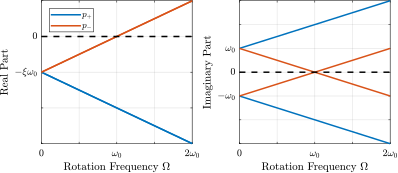
\includegraphics[scale=1]{figs/campbell_diagram.pdf}
\caption{\label{fig:campbell_diagram}Campbell Diagram}
\end{figure}

The magnitude of the coupling terms are increasing with the rotation speed.

\begin{figure}[htbp]
\centering
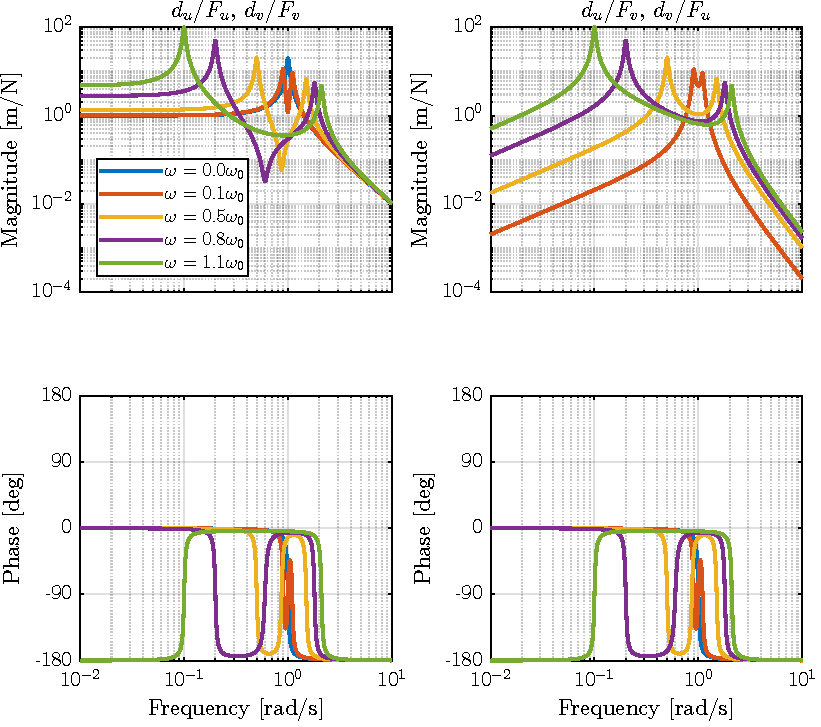
\includegraphics[scale=1]{figs/plant_compare_rotating_speed.pdf}
\caption{\label{fig:plant_compare_rotating_speed}Caption}
\end{figure}

\section{Integral Force Feedback}
\label{sec:org78c2eab}
\subsection{Control Schematic}
\label{sec:org6a00238}

\subsection{Equations}
\label{sec:org5480f1b}

\subsection{Plant Dynamics}
\label{sec:orgbb0952e}

\begin{figure}[htbp]
\centering
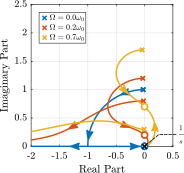
\includegraphics[scale=1]{figs/root_locus_pure_iff.pdf}
\caption{\label{fig:root_locus_pure_iff}Figure caption}
\end{figure}

\subsection{Physical Interpretation}
\label{sec:orgdb25e2c}

\section{Integral Force Feedback with Low Pass Filters}
\label{sec:org2985d35}

\begin{figure}[htbp]
\centering
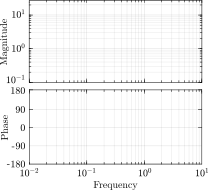
\includegraphics[scale=1]{figs/loop_gain_modified_iff.pdf}
\caption{\label{fig:loop_gain_modified_iff}Figure caption}
\end{figure}

\begin{figure}[htbp]
\centering
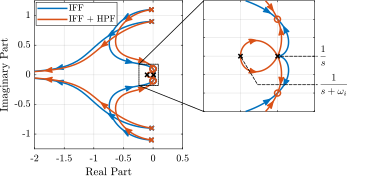
\includegraphics[scale=1]{figs/root_locus_modified_iff_bis.pdf}
\caption{\label{fig:root_locus_modified_iff}Figure caption}
\end{figure}

\begin{figure}[htbp]
\centering
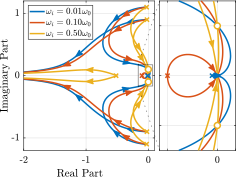
\includegraphics[scale=1]{figs/root_locus_wi_modified_iff.pdf}
\caption{\label{fig:root_locus_wi_modified_iff}Figure caption}
\end{figure}

\section{Integral Force Feedback with Parallel Springs}
\label{sec:orga4142a5}

\begin{figure}[htbp]
\centering
\includegraphics[scale=1]{figs/rotating_xy_platform_springs.pdf}
\caption{\label{fig:rotating_xy_platform_springs}Figure caption}
\end{figure}

\begin{figure}[htbp]
\centering
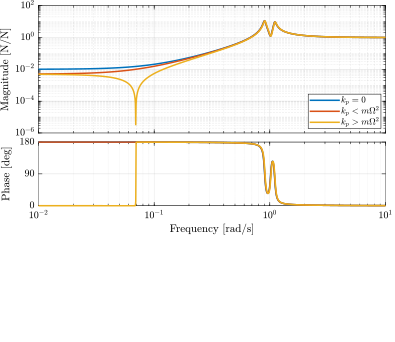
\includegraphics[scale=1]{figs/plant_iff_kp.pdf}
\caption{\label{fig:plant_iff_kp}Figure caption}
\end{figure}

\begin{figure}[htbp]
\centering
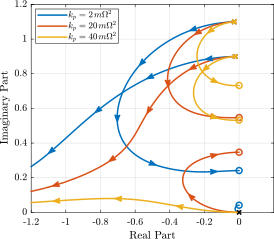
\includegraphics[scale=1]{figs/root_locus_iff_kps.pdf}
\caption{\label{fig:root_locus_iff_kps}Figure caption}
\end{figure}

\begin{figure}[htbp]
\centering
\includegraphics[scale=1]{figs/root_locus_iff_kp_bis.pdf}
\caption{\label{fig:root_locus_iff_kp_bis}Figure caption}
\end{figure}

\begin{figure}[htbp]
\centering
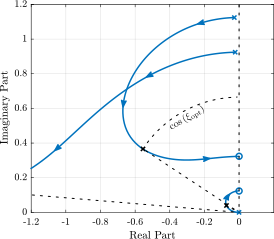
\includegraphics[scale=1]{figs/root_locus_opt_gain_iff_kp.pdf}
\caption{\label{fig:root_locus_opt_gain_iff_kp}Figure caption}
\end{figure}

\begin{figure}[htbp]
\centering
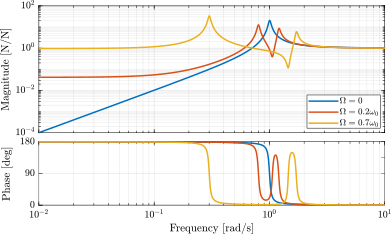
\includegraphics[scale=1]{figs/plant_iff_compare_rotating_speed.pdf}
\caption{\label{fig:plant_iff_compare_rotating_speed}Figure caption}
\end{figure}

\section{Direct Velocity Feedback}
\label{sec:org6a1be4f}

\begin{figure}[htbp]
\centering
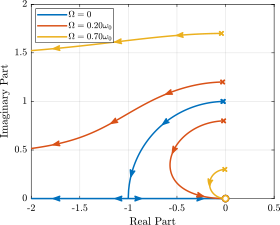
\includegraphics[scale=1]{figs/root_locus_dvf.pdf}
\caption{\label{fig:root_locus_dvf}Figure caption}
\end{figure}

\section{Comparison of the Proposed Active Damping Techniques}
\label{sec:orga9658c0}

\begin{figure}[htbp]
\centering
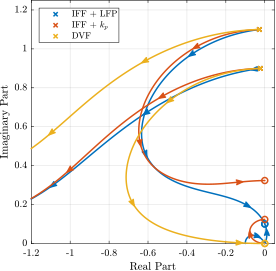
\includegraphics[scale=1]{figs/comp_root_locus.pdf}
\caption{\label{fig:comp_root_locus}Figure caption}
\end{figure}

\begin{figure}[htbp]
\centering
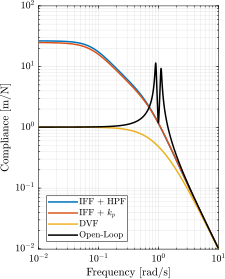
\includegraphics[scale=1]{figs/comp_compliance.pdf}
\caption{\label{fig:comp_compliance}Figure caption}
\end{figure}

\begin{figure}[htbp]
\centering
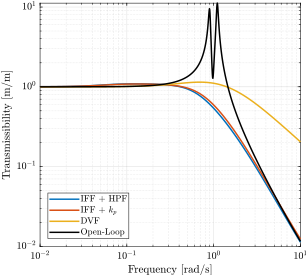
\includegraphics[scale=1]{figs/comp_transmissibility.pdf}
\caption{\label{fig:comp_transmissibility}Figure caption}
\end{figure}

\section{Conclusion}
\label{sec:orgcdf948f}
\label{sec:conclusion}


\section*{Acknowledgment}
\label{sec:org6c21e13}

\bibliography{ref.bib}
\end{document}
